实例化如图 \ref{fig:a-sample} 所示的DFA,测试代码如代码 \ref{lst:a-sample} 所示

% \begin{figure}
	% \centering
	% 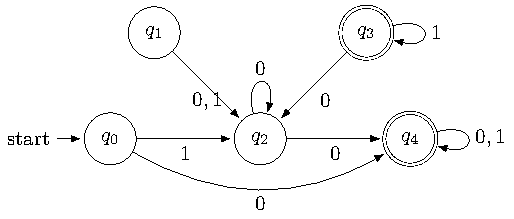
\includegraphics[width=0.8\textwidth]{automaton.tex}
	% \caption{}
	% \label{fig:a-sample}
% \end{figure}

\begin{figure}[!htbp]
	\centering
	\resizebox {0.9\textwidth} {!} {
		\begin{tikzpicture}[>=latex, shorten >=2pt,node distance=1in, on grid, auto]
			\node[state,initial] (q0) {$q_0$};
			\node[state] (q2) [right=of q0] {$q_2$};
			\node[state,accepting] (q4) [right=of q2] {$q_4$};
			\node[state] (q1) [above left=of q2] {$q_1$};
			\node[state,accepting] (q3) [above right=of q2] {$q_3$};
			\path[->]
			(q0) edge [below,bend right] node {$0$} (q4)
			(q2) edge [below] node {$0$} (q4)
			(q0) edge [below] node {$1$} (q2)
			(q1) edge [below] node {$0,1$} (q2)
			(q3) edge node {$0$} (q2)
			(q2) edge [loop above] node {$1$} (q2)
			(q4) edge [loop right] node {$0,1$} (q4)
			(q3) edge [loop right] node {$1$} (q3)
			;
		\end{tikzpicture}
    }
	\caption{}
	\label{fig:a-sample}
\end{figure}

\begin{lstlisting}[language=C++,label={lst:a-sample},caption={图 \ref{fig:a-sample} 中的DFA}]
void minDFATest3()
{
	DFA_components dfa_com1;

	// StateSet S  开始状态集
	dfa_com1.S.set_domain(5);
	dfa_com1.S.add(0);

	// StateSet F  结束状态集
	dfa_com1.F.set_domain(5);
	dfa_com1.F.add(3);
	dfa_com1.F.add(4);

	int i = 5;
	while (i--)
	{
		dfa_com1.Q.allocate();
	}

	dfa_com1.T.set_domain(5);
	dfa_com1.T.add_transition(0, '0', 4);
	dfa_com1.T.add_transition(0, '1', 2);
	dfa_com1.T.add_transition(1, '0', 2);
	dfa_com1.T.add_transition(1, '1', 2);
	dfa_com1.T.add_transition(2, '0', 4);
	dfa_com1.T.add_transition(2, '1', 2);
	dfa_com1.T.add_transition(3, '0', 2);
	dfa_com1.T.add_transition(3, '1', 3);
	dfa_com1.T.add_transition(4, '0', 4);
	dfa_com1.T.add_transition(4, '1', 4);

	//实例化一个DFA对象
	DFA dfa1(dfa_com1);
	cout << "\n************ DFA\n" << std::flush;
	cout << dfa1 << endl;

	dfa1.usefulf();  // 没有删除1,3 ?
	cout << dfa1 << endl;
	cout << " is the DFA Usefulf ?: " << dfa1.Usefulf() << endl;

	dfa1.min_Hopcroft();
	cout << "\n************ minDFA\n" << std::flush;
	cout << dfa1 << endl;
}
\end{lstlisting}

代码 \ref{lst:a-sample} 将输出如下信息

\begin{lstlisting}[language=C++,label={lst:a-sample-result},caption={图 \ref{fig:a-sample} 中的DFA 在算法 Hopcroft 算法中的输出}]
************ DFA

DFA
Q = [0,5)
S = { 0 }
F = { 3  4 }
Transitions =
0->{ '0'->4  '1'->2 }
1->{ ['0','1']->2 }
2->{ '0'->4  '1'->2 }
3->{ '0'->2  '1'->3 }
4->{ ['0','1']->4 }

current = -1


DFA
Q = [0,5)
S = { 0 }
F = { 3  4 }
Transitions =
0->{ '0'->4  '1'->2 }
1->{ ['0','1']->2 }
2->{ '0'->4  '1'->2 }
3->{ '0'->2  '1'->3 }
4->{ ['0','1']->4 }

current = -1

 is the DFA Usefulf ?: 1

************ minDFA

DFA
Q = [0,4)
S = { 0 }
F = { 2  3 }
Transitions =
0->{ '0'->3  '1'->0 }
1->{ ['0','1']->0 }
2->{ '0'->0  '1'->2 }
3->{ ['0','1']->3 }
current = -1
\end{lstlisting}

本例中,$q_1$和$q_3$都不是 \verb+final-unreachable+ (陷阱)状态,所以不会在执行函数 \verb+DFA::usefulf()+ 后去除。

执行最小化算法 \verb+DFA::min_Hopcroft+ 后的 DFA 如图 \ref{fig:a-sample-error} 所示。

\begin{figure}[!htbp]
	\centering
	\resizebox {0.6\textwidth} {!} {
		\begin{tikzpicture}[>=latex, shorten >=2pt,node distance=1in, on grid, auto]
			\node[state,initial] (q0) {$q_0$};
			\node[state,accepting]  [right=of q0] (q3) {$q_3$};
			\node[state,accepting]  [above=of q3] (q2) {$q_2$};
			\node[state] [left =of q2] (q1) {$q_1$};
			\path[->]
			(q0) edge [below] node {$0$} (q3)
			(q0) edge [loop below] node {$1$} (q0)
			(q1) edge  node {$0,1$} (q0)
			(q2) edge [below] node {$0$} (q0)
			(q2) edge [loop right] node {$1$} (q2)
			(q3) edge [loop right] node {$0,1$} (q3)
			;
		\end{tikzpicture}
    }
	\caption{}
	\label{fig:a-sample-error}
\end{figure}

经过测试,算法\verb+DFA::min_dragon+,\verb+DFA::min_Watson+,\verb+DFA::min_HopcroftUllman+的输出与算法\verb+DFA::min_Hopcroft+相同。而算法\verb+DFA::min_Brzozowski+的输出为
\begin{lstlisting}[language=C++,label={lst:a-sample-Brzozowski},caption={图 \ref{fig:a-sample} 中的DFA 在算法 Hopcroft 算法中的输出}]
************ DFA
DFA
Q = [0,2)
S = { 0 }
F = { 1 }
Transitions =
0->{ '0'->1  '1'->0 }
1->{ ['0','1']->1 }

current = -1
\end{lstlisting}

对应的状态转移图为图 \ref{fig:a-sample-bbb}

\begin{figure}[!htbp]
	\centering
	\resizebox {0.5\textwidth} {!} {
		\begin{tikzpicture}[>=latex, shorten >=2pt,node distance=1in, on grid, auto]
			\node[state,initial] (q0) {$q_0$};
			\node[state,accepting]  [right=of q0] (q1) {$q_1$};
			\path[->]
			(q0) edge [below] node {$0$} (q1)
			(q0) edge [loop above] node {$1$} (q0)
			(q1) edge [loop above] node {$0,1$} (q1)
			;
		\end{tikzpicture}
    }
	\caption{}
	\label{fig:a-sample-bbb}
\end{figure}

\newpage

{\bfseries 结论}

对于图 \ref{fig:a-sample} 中的自动机,仅有算法 \verb+DFA::min_Brzozowski+输出了正确的结果,\verb+DFA::min_Hopcroft+无论是否经过修改,均输出错误结果。

对于图 \ref{fig:a-sample} 中的自动机,移除状态$q_3$之后,之前错误的算法也能输出正确结果。

\begin{remark}
除了算法\verb+DFA::min_Brzozowski+外,其他算法均不能移除自动机中的开始不可达状态。
\end{remark}

增加对其他算法的测试后的代码如下
\begin{lstlisting}[language=C++,label={lst:a-sample-addtion},caption={}]
void minDFATest3()
{
	DFA_components dfa_com1;

	// StateSet S  开始状态集
	dfa_com1.S.set_domain(5);
	dfa_com1.S.add(0);

	// StateSet F  结束状态集
	dfa_com1.F.set_domain(5);
	dfa_com1.F.add(3);
	dfa_com1.F.add(4);

	int i = 5;
	while (i--)
	{
		dfa_com1.Q.allocate();
	}

	dfa_com1.T.set_domain(5);
	dfa_com1.T.add_transition(0, '0', 4);
	dfa_com1.T.add_transition(0, '1', 2);
	dfa_com1.T.add_transition(1, '0', 2);
	dfa_com1.T.add_transition(1, '1', 2);
	dfa_com1.T.add_transition(2, '0', 4);
	dfa_com1.T.add_transition(2, '1', 2);
	dfa_com1.T.add_transition(3, '0', 2);
	dfa_com1.T.add_transition(3, '1', 3);
	dfa_com1.T.add_transition(4, '0', 4);
	dfa_com1.T.add_transition(4, '1', 4);

	//实例化一个DFA对象
	DFA dfa1(dfa_com1);
	cout << "\n************ DFA\n" << std::flush;
	cout << dfa1 << endl;

	cout << " is the DFA Usefulf ?: " << dfa1.Usefulf() << endl;
	dfa1.usefulf();  // 没有删除1,3 ?
	cout << dfa1 << endl;
	cout << " is the DFA Usefulf ?: " << dfa1.Usefulf() << endl;

	dfa1.min_Hopcroft();
	cout << "\n************ minDFA (Hopcroft) \n" << std::flush;
	cout << dfa1 << endl;


	//增加对其他最小化算法的测试
	DFA dfa2(dfa_com1);
	dfa2.min_Brzozowski();
	cout << "\n************ minDFA (Brzozowski)\n" << std::flush;
	cout << dfa2 << endl;

	DFA dfa3(dfa_com1);
	dfa3.usefulf();
	dfa3.min_dragon();
	cout << "\n************ minDFA (dragon) \n" << std::flush;
	cout << dfa3 << endl;

	DFA dfa4(dfa_com1);
	dfa4.usefulf();
	dfa4.min_HopcroftUllman();
	cout << "\n************ minDFA (HopcroftUllman) \n" << std::flush;
	cout << dfa4 << endl;

	DFA dfa5(dfa_com1);
	dfa5.usefulf();
	dfa5.min_Watson();
	cout << "\n************ minDFA (Watson)\n" << std::flush;
	cout << dfa5 << endl;
}
\end{lstlisting}